\section{Deskripsi Tugas}

Tugas kecil ini berfokus pada pembuatan \textit{solver} untuk permainan \textit{Ice Sliding Puzzle}. Program menerima sebuah papan permainan berbentuk $N \times M$ dari berkas teks, kemudian mencari urutan gerakan yang membawa pin dari posisi awal \texttt{Z} ke tujuan \texttt{O}. Selama pencarian, pin hanya dapat bergerak ke empat arah utama, dan karena lantai bersifat licin, pin akan terus meluncur sampai tertahan oleh dinding atau batu \texttt{X}.

Selain mencapai tujuan, solusi yang valid juga harus melewati angka-angka pada papan secara berurutan lengkap, mulai dari \texttt{0} hingga angka terbesar yang tersedia. Apabila pin melewati lava \texttt{L}, keluar dari batas papan, atau menginjak angka di luar urutan, maka keadaan tersebut dianggap gagal. Dengan demikian, program tidak hanya mencari jalur terpendek atau termurah, tetapi juga jalur yang mematuhi seluruh aturan permainan.

Gambar berikut memperlihatkan contoh papan permainan beserta legenda simbol yang digunakan pada laporan ini.

\begin{figure}[H]
    \centering
    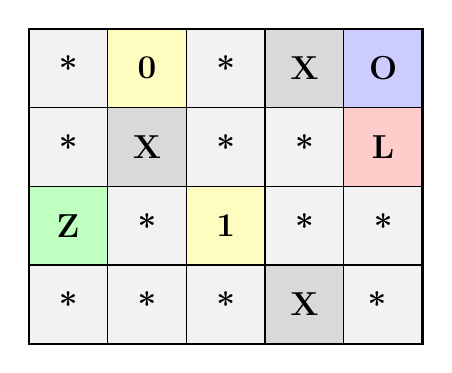
\begin{tikzpicture}[
            x=1cm,
            y=1cm,
            board cell/.style={draw, line width=0.45pt, minimum size=1cm, inner sep=0pt, outer sep=0pt, align=center, font=\large\bfseries}
        ]
        \foreach \x/\y/\fillcolor/\value in {
                0/0/gray!10/*,
                1/0/yellow!25/0,
                2/0/gray!10/*,
                3/0/black!15/X,
                4/0/blue!20/O,
                0/1/gray!10/*,
                1/1/black!15/X,
                2/1/gray!10/*,
                3/1/gray!10/*,
                4/1/red!20/L,
                0/2/green!25/Z,
                1/2/gray!10/*,
                2/2/yellow!25/1,
                3/2/gray!10/*,
                4/2/gray!10/*,
                0/3/gray!10/*,
                1/3/gray!10/*,
                2/3/gray!10/*,
                3/3/black!15/X,
                4/3/gray!10/*
            } {
                \node[board cell, fill=\fillcolor] at (\x+0.5,3.5-\y) {\value};
            }
        \draw[line width=0.8pt] (0,0) rectangle (5,4);
    \end{tikzpicture}
    \caption{Contoh visualisasi papan \textit{Ice Sliding Puzzle}.}
    \label{fig:contoh-papan-ice-sliding}
\end{figure}

\noindent
Pada contoh di atas, simbol \texttt{Z} menandai posisi awal, \texttt{O} menandai tujuan, \texttt{X} adalah rintangan, \texttt{L} adalah lava, sedangkan \texttt{0} dan \texttt{1} adalah angka yang harus dilewati secara berurutan sebelum pin dapat dinyatakan menang. Tile bertanda \texttt{*} merepresentasikan jalur kosong yang dapat dilewati pin.

\section{Spesifikasi Program}
\begin{itemize}
    \item  Buatlah sebuah program tersebut dalam bahasa Java, Python, C++, C, atau GO yang mengimplementasikan algoritma Pathfinding (UCS, GBFS, dan A*) untuk mencari solusi dalam permainan Ice Sliding Puzzle Solver.
    \item Tugas dikerjakan berkelompok dengan anggota maksimal 2 orang, boleh lintas kelas maupun kampus. Silahkan isi pendataan kelompok pada link berikut.
    \item  \textbf{Input}: program akan memberikan pengguna sebuah arahan pada terminal (jika tidak mengerjakan bonus) untuk memilih file test case berekstensi .txt, kemudian program membaca file test case tersebut yang berisi konfigurasi awal dari map Permainan yang akan diselesaikan. Perhatikan bahwa input dapat memiliki ukuran papan yang berbeda-beda (tidak harus persegi), serta program harus dapat memvalidasi apakah input yang diberikan merupakan input valid atau bukan.
\end{itemize}

Contoh perhitungan cost gerakan adalah sebagai berikut.
\begin{itemize}
    \item Misalkan aktor melakukan satu gerakan ke kanan dan selama gerakan tersebut melewati tiga tile dengan cost berturut-turut: 2, 5, dan 4. Maka cost gerakan itu adalah $2 + 5 + 4 = 11$.
    \item Total cost solusi adalah jumlah dari semua cost gerakan yang dilakukan sepanjang solusi.
    \item Perlu diingat: tile `X` dan `L` tetap mempunyai nilai cost dalam input, tetapi tidak dihitung dalam solusi valid karena `X` tidak pernah dilewati dan `L` menyebabkan game over jika dilewati.
\end{itemize}

\begin{tcolorbox}[
        colback=black!3,
        colframe=black!60,
        boxrule=0.6pt,
        left=1mm,
        right=1mm,
        top=1mm,
        bottom=1mm,
        listing only,
        listing options={basicstyle=\ttfamily\small, columns=fullflexible, keepspaces=true}
    ]
    Contoh: \\
    Gerakan 1: tiles traversed costs = 2, 5, 4, maka movement cost = 11 \\
    Gerakan 2: tiles traversed costs = 3, 2, maka movement cost = 5 \\
    Total cost solusi = $11 + 5 = 16$
\end{tcolorbox}

\section{Output}

Program harus menghasilkan keluaran berikut setelah pencarian selesai:
\begin{enumerate}
    \item Menampilkan solusi gerakan yang ditemukan (mis. RULUDR...).
    \item Menampilkan total cost dari solusi.
    \item Menampilkan visualisasi papan pada solusi, yaitu keadaan papan sehingga aktor dapat mencapai titik \texttt{O} menggunakan algoritma pathfinding yang dipilih. Visualisasi ini harus menandai lintasan akhir yang ditempuh aktor.
    \item Menampilkan jumlah konfigurasi / iterasi yang ditinjau oleh algoritma. Program harus menyediakan opsi untuk menyimpan setiap iterasi (state) ke file berekstensi \texttt{.txt} sehingga dapat dianalisis atau diputar ulang nanti.
    \item Menampilkan waktu eksekusi algoritma dalam milidetik. Pengukuran waktu harus meliputi hanya waktu komputasi (search), tidak termasuk waktu I/O membaca/menulis file.
    \item Playback (bukan live update), dimana setelah algoritma selesai, program harus dapat memvisualisasikan proses pathfinding sebagai rangkaian langkah yang dapat diputar mundur/maju. Contoh playback di CLI dapat berisi fitur-fitur di bawah ini.
          \begin{enumerate}
              \item Arrow kiri/kanan untuk mundur/maju satu step.
              \item ESC: prompt user untuk memasukkan nomor step X dan langsung lompat ke step tersebut.
          \end{enumerate}
\end{enumerate}

Catatan: untuk mode GUI (bonus), playback harus memiliki kontrol kecepatan (play/pause/seek) dan kemampuan maju/mundur yang setara dengan pengalaman video. Berikut adalah contoh file .txt yang akan dijadikan sebagai input.
\\ \\
Baris pertama memuat 2 angka $(N, M)$ yang menyatakan panjang dan lebar papan \\
N baris berikutnya merepresentasikan papan \\
N baris berikutnya merepresentasikan cost untuk melewati tile tersebut \\

\begin{tcolorbox}[
        title=Contoh Input,
        listing only,
        enhanced,
        sharp corners,
        colback=black!2,
        colframe=black!70,
        boxrule=0.7pt,
        fonttitle=\bfseries\small,
        left=2mm,
        right=2mm,
        top=1mm,
        bottom=1mm,
        listing options={basicstyle=\ttfamily\footnotesize, columns=fullflexible, keepspaces=true, breaklines=false, showstringspaces=false, showtabs=false, tabsize=2}
    ]
    7 7 \\
    XXXXXXX \\
    X0****X \\
    X**X**X \\
    X****OX \\
    X***1LX \\
    XZ**X*X \\
    XXXXXXX \\
    999 999 999 999 999 999 999 \\
    999 3 5 2 8 1 999 \\
    999 7 4 999 6 9 999 \\
    999 2 8 3 5 4 999 \\
    999 6 1 7 2 999 999 \\
    999 9 3 4 999 8 999 \\
    999 999 999 999 999 999 999 \\
\end{tcolorbox}

\noindent
Keterangan:
\begin{itemize}
    \item \texttt{*} = path yang bisa dilewati.
    \item \texttt{X} = Rintangan/Batu. Aktor akan berhenti tepat sebelum batu.
    \item \texttt{L} = Lava. Melewati lava akan mengalami game over (meskipun tidak berhenti tepat di lava).
    \item \texttt{Z} = Aktor/Pengguna.
    \item \texttt{O} = Titik tujuan.
    \item \texttt{<i>} = Angka. Ini adalah modifikasi pada spesifikasi tugas. Aktor harus melewati angka-angka ini sesuai urutan yang ada pada papan. Petak berangka 1 harus dilewati setelah aktor melewati petak berangka 0. petak berangka 2 harus dilewati setelah petak berangka 1 dan seterusnya (maksimal sampai 9).
\end{itemize}

\noindent
Aturan tambahan yang penting.
\begin{itemize}
    \item Jika aktor menginjak angka di luar urutan (mis.\, menginjak 1 sebelum 0), maka kondisi tersebut dianggap game over.
    \item Setelah sebuah petak angka dilewati sesuai urutan, petak tersebut berubah menjadi petak biasa dan dapat dilalui lagi tanpa batasan urutan.
    \item Petak angka adalah tile normal (bukan rintangan). Akibatnya, aktor akan meluncur melewatinya jika bergerak tanpa berhenti.
    \item Jika aktor bergerak menuju sisi papan (kanan/atas/kiri/bawah) dan tidak ada rintangan pada sisi tersebut untuk menghentikannya, maka aktor akan keluar papan dan kondisi dianggap game over. Dengan demikian, permainan harus diulang dari awal.
    \item Pin/aktor harus tepat berhenti pada titik \texttt{O} dan semua angka harus telah dilewati sesuai urutan agar kondisi dianggap sukses.
    \item Setiap tile memiliki cost traversal yang diberikan pada bagian kedua input. Cost merepresentasikan biaya ketika aktor melewati suatu tile.
    \item Cost gerakan dihitung dari jumlah cost seluruh tile yang dilalui selama satu gerakan sliding. Tile posisi awal pada awal gerakan tidak dihitung, tetapi tile tempat aktor berhenti pada akhir gerakan tetap dihitung.
\end{itemize}

\section{Spesifikasi Bonus}

Poin maksimal untuk bonus adalah 10. Mahasiswa dapat memilih satu atau beberapa spesifikasi bonus di bawah ini; total poin tambahan yang diberikan untuk tugas tidak boleh melebihi 10 poin.

\begin{enumerate}
    \item \textbf{GUI penuh untuk program (maks 6 poin)}. Membuat antarmuka grafis yang memungkinkan pengguna memilih file input, menampilkan papan, mengatur kecepatan playback, dan memutar langkah mundur/maju. Kriteria penilaian:

    \item \textbf{Tambahkan algoritma pathfinding tambahan (maks 2 poin)}. Implementasi setidaknya satu algoritma pathfinding lain selain yang diwajibkan (mis.\, Dijkstra, IDA*, BFS adaptif untuk sliding puzzle, atau algoritma lain yang relevan). Penilaian:

    \item \textbf{Tambahkan dua alternatif heuristik (maks 2 poin)}. Sediakan dua heuristik tambahan untuk A* selain heuristik utama. Kriteria:

    \item \textbf{Optimasi kecepatan pencarian (maks 5 poin, tetapi total bonus tetap dibatasi)}. Optimasi yang dapat meningkatkan kecepatan menemukan solusi. Penilaian didasarkan pada bukti eksperimen dan metrik yang jelas.
\end{enumerate}

Catatan penting tentang pemberian nilai.
\begin{itemize}
    \item Total poin bonus yang diberikan tidak boleh melebihi 10, meskipun jumlah maksimum per-item jika dijumlahkan lebih besar. Dosen/TA akan memilih kombinasi fitur yang memberi nilai maksimal hingga 10 poin.
    \item Untuk setiap fitur bonus, sertakan bukti fungsionalitas: screenshot GUI atau rekaman pendek (untuk GUI), hasil benchmark (untuk kecepatan), dan contoh keluaran atau log yang menunjukkan algoritma/heuristik baru bekerja.
    \item Semua kode bonus harus disertakan pada repositori akhir dan dilengkapi instruksi build/run di README.
\end{itemize}

Instruksi pengumpulan bonus.
\begin{itemize}
    \item Sertakan penjelasan singkat di README tentang fitur bonus yang diimplementasikan dan bagaimana mengaktifkannya (mis.\, argumen CLI atau flag pada GUI).
    \item Apabila mengumpulkan GUI, sertakan screenshot dan langkah untuk menjalankan (dependensi, command build, dan cara membuka file input).
\end{itemize}

